
% =========================================================================================
% HOMEWORK TEMPLATE %===================================================================
% =========================================================================================

% =========================================================================================
% LaTeX SETUP %============================================================================
% =========================================================================================
\documentclass{report}						% Change "article" to "report" to get rid of page number on title page
\usepackage{amsmath,amsfonts,amsthm,amssymb,empheq}
\usepackage{setspace}
\usepackage{Tabbing}
\usepackage{fancyhdr}
\usepackage{lastpage}
\usepackage{extramarks}
\usepackage{chngpage}
\usepackage{soul,color}
\usepackage{graphicx,float,wrapfig}
\usepackage[retainorgcmds]{IEEEtrantools}

% =========================================================================================
% TikZ SETUP %==============================================================================
% =========================================================================================
\usepackage{tikz}
\usepackage{verbatim}
\usetikzlibrary{shapes,arrows,positioning,calc,scopes,angles,quotes}
\usetikzlibrary{decorations.markings}

% =========================================================================================
% MARGINS %===============================================================================
% =========================================================================================
\topmargin=-0.45in      
\evensidemargin=0in     
\oddsidemargin=0in      
\textwidth=6.5in        
\textheight=9.0in       
\headsep=0.25in         

% =========================================================================================
% ASSIGNMENT INFORMATION %===============================================================
% =========================================================================================
\newcommand{\hmwkTitle}{Homework\ \#5}
\newcommand{\hmwkDueDate}{ March\ 9,\ 2016}
\newcommand{\hmwkClass}{EE\ 324}
\newcommand{\hmwkClassTime}{Munk}
\newcommand{\hmwkClassInstructor}{Prof. Jens}
\newcommand{\hmwkAuthorName}{Blair Munro}

% =========================================================================================
% HEADER & FOOTER %=======================================================================
% =========================================================================================
\pagestyle{fancy}                                                       
\lhead{\hmwkAuthorName}                                                 
\chead{\hmwkClass\ (\hmwkClassInstructor\ \hmwkClassTime): \hmwkTitle}  
\rhead{\firstxmark}                                                     
\lfoot{\lastxmark}                                                      
\cfoot{}                                                                
\rfoot{Page\ \thepage\ of\ \pageref{LastPage}}                          
\renewcommand\headrulewidth{0.4pt}                                      
\renewcommand\footrulewidth{0.4pt}                                      

% =========================================================================================
% CUSTOM MATH COMMANDS %================================================================
% =========================================================================================
\newcommand{\ud}{\,\mathrm{d}}						%creates roman-script differential d , with added space
\newcommand{\pd}[2]{\frac {\partial #1}{\partial #2}} 										%partial derivative
\newcommand{\td}[2]{\frac {\mathrm{d} #1}{\mathrm{d} #2}}									  %derivative
\newcommand{\tdd}[2]{\frac {\mathrm{d}^2 #1}{\mathrm{d} #2^2}}  						      %second derivative
\newcommand{\val}[2]{#1 \text{ #2}}							 	    %formats a numerical value with text units
\newcommand{\comm}[1]{\text{#1}\qquad}
% =========================================================================================
% MAKE TITLE %=============================================================================
% =========================================================================================
\title{\vspace{2in}\textmd{\textbf{\hmwkClass:\ \hmwkTitle}}\\\normalsize\vspace{0.1in}\small{Due\ on\hmwkDueDate}\\\vspace{0.1in}\large{\textit{\hmwkClassInstructor\ \hmwkClassTime}}\vspace{3in}}
\date{}
\author{\textbf{\hmwkAuthorName}}

% =========================================================================================
% BEGIN DOCUMENT %=======================================================================
% =========================================================================================

\begin{document}
\begin{spacing}{1.1}
\maketitle

\newpage
\begin{enumerate}
%PROBLEMS ================================================================================
\item[{\bf \large 1.}] 
%	1
Match the load $Z_L=20+j40\Omega$ to a $Z_C=50\Omega$ transmission line.
\begin{figure}[!hbp]
\centering
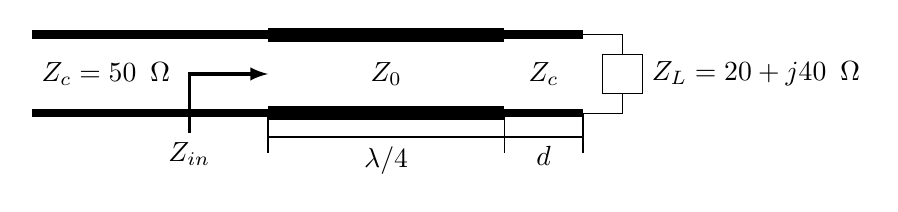
\begin{tikzpicture}[
	scale=1,
	vector/.style={very thick,->, >=latex},
	axis/.style={very thick, ->, >=stealth'}]
		\draw[line width=3pt] (-3,1)--(4,1);
		\draw[line width=3pt] (-3,0)--(4,0);
		\draw (4,1)--(4.5,1)--(4.5,0)--(4,0);
		\draw[fill=white] (4.25,0.75) rectangle (4.75,0.25);
		\draw (4.75,0.5) node[right]{$Z_L=20+j40\enspace\Omega$};
		\draw (-3,0.5) node[right]{$Z_c=50\enspace\Omega$};
		\draw[vector] (-1,-0.25)|-(0,0.5);
		\draw (-1,-0.25) node[below]{$Z_{in}$};
		\draw[line width=5pt] (0,1)--(3,1);
		\draw[line width=5pt] (0,0)--(3,0);
		\draw (0,0)--(0,-.5) (3,0)--(3,-0.5) (4,0)--(4,-.5) (0,-0.30)--(4,-0.3) ;
		\draw (1.5,-0.30) node [below] {$\lambda/4$} (3.5,-0.30) node [below] {$d$};
		\draw (3.5,0.5) node{$Z_c$};
		\draw (1.5,0.5) node{$Z_0$};
\end{tikzpicture}
\caption{Problem 1, quarter wave transform, transmission line model.}
\end{figure}
\subitem{\bf\large (a)} What is the shortest length $d$ such that the impedance attached to the quarter wave section is purely real?
\begin{IEEEeqnarray*}{lrCl}
\comm{normalized impedances}&
z_L&=&0.4+j0.8\Omega \\
\comm{from smith chart}&
d&=&(0.250-0.114)\lambda \\
\end{IEEEeqnarray*}
shortest length $d$ is \[\boxed{d=0.136\lambda}\]
\subitem{\bf\large (b)} What characteristic impedance value to we require for the quarter wave section?
\begin{IEEEeqnarray*}{lrCl}
\comm{from smith chart,}&
z_1&\approx&	4.3\Omega	\\
\comm{un-normalized,}&
Z_1&=&	215\Omega	\\
\comm{so we require}&
Z_0	&=&	\sqrt{Z_1Z_c}	\\
\comm{}&
&=&	\sqrt{(215)(50)}	\\
\end{IEEEeqnarray*}
\[\boxed{Z_0=103.7\Omega}\]
\begin{figure}[!hbp]
\centering
\begin{tikzpicture}[
	scale=1,
	vector/.style={very thick,->, >=latex},
	axis/.style={very thick, ->, >=stealth'}]
		%	SMITH CHART: 
		%	2.34pt/mm	210pt, outer-mid	201pt, outer-inmid	225pt, outer	192pt, inner	
		%	[thick](90:226pt)--(90:238pt)		
		\node[inner sep=0pt] (russell) at (0,0){\includegraphics[width=1\textwidth]{SMITHCHARTSCAN.jpg}};
		\begin{scope}[shift={(-4.8pt,35.2pt)}]

			\draw[dashed, red, very thick] (0,0)--(97.25:250pt);
			\draw[red] (97.25:250pt) node [right]{0.114};
			\draw[fill=green] (97.25:119pt) circle(2pt) (97.25:119pt) node [right]{$\mathbf{z_L}$};
			\draw[dashed, red, very thick] (0,0)--(0:250pt);
			\draw[red] (0:250pt) node [right]{0.250};
			\draw[fill=green] (0:119pt) circle(2pt) (0:119pt) node [below]{$\mathbf{z_1}$};
			\draw[red, vector, very thick] (60:250pt) arc (60:30:250pt);

		\end{scope}
\end{tikzpicture}
\caption{Problem 1, Smith Chart.}
\end{figure}
%	2
\newpage
\item[{\bf \large 2.}] 
Use a parallel single stub tuner to match the load $Z_L=120+j30 \Omega$ to a 50 ohm transmission line.
\begin{figure}[!hbp]
\centering
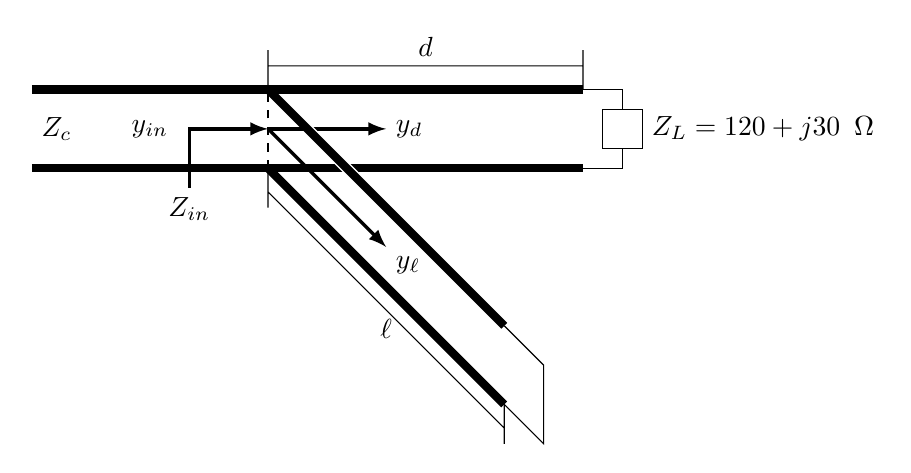
\begin{tikzpicture}[
	scale=1,
	vector/.style={very thick,->, >=latex},
	axis/.style={very thick, ->, >=stealth'}]
		\draw[line width=3pt] (-3,1)--(4,1);
		\draw[line width=3pt] (-3,0)--(4,0);
		\draw (4,1)--(4.5,1)--(4.5,0)--(4,0);
		\draw[fill=white] (4.25,0.75) rectangle (4.75,0.25);
		\draw (4.75,0.5) node[right]{$Z_L=120+j30\enspace\Omega$};
		\draw (-3,0.5) node[right]{$Z_c$};
		\draw (-1.5,0.5) node{$y_{in}$};
		\draw[vector] (-1,-0.25)|-(0,0.5);
		\draw (-1,-0.25) node[below]{$Z_{in}$};
		\draw [vector] (0,.5)--(1.5,.5);
		\draw[white,line width=4pt] (.5,.5)--(3,-2);
		\draw[line width=3pt] (0,1)--(3,-2);
		\draw[line width=3pt] (0,0)--(3,-3);
		\draw (3,-3)--(3.5,-3.5)--(3.5,-2.5)--(3,-2);
		\draw (0,0)--(0,-.5) (3,-3)--(3,-3.5) (0,1)--(0,1.5) (4,1)--(4,1.5) (4,1.3)--(0,1.3) (0,-0.3)--(3,-3.3);
		\draw (2,1.3) node [above] {$d$} (1.5,-1.8) node [below] {$\ell$};
		\draw[dashed] (0,0)--(0,1);
		\draw[vector] (0,0.5)--(1.5,-1);
		\draw (1.5,-1) node [below right] {$y_\ell$};
		\draw (1.5,0.5) node [right]{$y_d$};
		
\end{tikzpicture}
\caption{Problem 2, parallel single stub tuner.}
\end{figure}
\subitem{\bf\large (a)} If all the sections of this line are 50 ohm, determine the lengths $d$ and $\ell$ required to match the load.
\begin{IEEEeqnarray*}{lrCl}
\comm{normalized load}&
z_L&=&2.4+j0.6 \Omega	\\
\comm{match load requires}&
y_d&=&1+jB	\\
\comm{we also know}&
y_{in}&=&	y_d+y_\ell\\
\comm{from smith chart}&
y_d&=&1 +j	\\
\comm{therefore we require}&
y_\ell&=&-j	\\
\comm{plot and rotate to short}&
&&	\\
\comm{thus (from Smith Chart)}&
d&=&((0.5-0.482)+0.162)\lambda	\\
\comm{}&
\ell&=&\lambda/8	\\
\end{IEEEeqnarray*}
\[\boxed{ d=0.180\lambda \qquad \ell=0.125\lambda}\]
\subitem{\bf\large (b)} Repeat the above, but this time for a stud characteristic impedance of 100 ohms.

In this case, everything remains the same, except this time the admittance we require for $y_\ell$ after renormalizing to the new characteristic impedance is $j2$.

From the Smith Chart, $\ell=(0.25-0.176)\lambda$

\[\boxed{ d=0.180\lambda \qquad \ell=0.074\lambda}\]
\begin{figure}[!hbp]
\centering
\begin{tikzpicture}[
	scale=1,
	vector/.style={very thick,->, >=latex},
	axis/.style={very thick, ->, >=stealth'}]
		%	SMITH CHART: 
		%	2.34pt/mm	210pt, outer-mid	201pt, outer-inmid	225pt, outer	192pt, inner	
		%	[thick](90:226pt)--(90:238pt)		
		\node[inner sep=0pt] (russell) at (0,0){\includegraphics[width=1\textwidth]{SMITHCHARTSCAN.jpg}};
		\begin{scope}[shift={(-4.8pt,35.2pt)}]
			\draw[dashed, red, very thick] (0,0)--(13.25:250pt) (0,0)--(13.25-180:250pt);
			\draw[red] (13.25-180:250pt) node [left]{0.482};
			\draw[fill=green] (13.25:84.5pt) circle(2pt) (13.25:84.5pt) node [below]{$\mathbf{z_L}$};
			\draw[fill=yellow ] (13.25-180:84.5pt) circle(2pt) (13.25-180:84.5pt) node [below]{$\mathbf{y_L}$};
			\draw[red, vector, very thick] (180:250pt) arc (180:150:250pt) ;
			\draw[red, vector, very thick] (-80:250pt) arc (-80:-60:250pt);
			\draw[dashed, red, very thick] (13.25-180:84.5pt) arc (13.25-180:13.25-310:84.5pt);
			\draw[dashed, red, very thick] (0,0)--(13.25-310:250pt);
			\draw[red] (13.25-310:250pt) node [above]{0.162};
			\draw[red] (-53:250pt) node [right]{0.176};
			\draw[fill=yellow ] (13.25-310:84.5pt) circle(2pt) (13.25-310:84.5pt) node [right]{$\mathbf{y_d}$};
			\draw[dashed, red, very thick] (0,0)--(-90:250pt) (0,0)--(0:250pt) (0,0)--(-53:250pt);
			\draw[dashed, red, very thick] (-90:192pt) arc (-90:0:192pt);
			\draw[fill=yellow ] (-90:192pt) circle(2pt) (-90:192pt) node [right]{$\mathbf{y_\ell}$};
			\draw[fill=yellow ] (0:192pt) circle(2pt) (0:192pt) node [below]{$\mathbf{short}$};
			\draw[fill=yellow ] (-53:192pt) circle(2pt) (-53:192pt) node [right]{$\mathbf{y_\ell}$};
		\end{scope}
\end{tikzpicture}
\caption{Problem 2, Smith Chart.}
\end{figure}
\newpage
%	3
\item[{\bf \large 3.}]
The parallel double stub method is used to match a load impedance of $Z_L=200+j200\Omega$ to a lossless transmission line of characteristic impedance $Z_c=100\Omega$. The spacing between the stubs is $0.1\lambda$, and one stub is connected directly in parallel with the load.
\subitem{\bf\large (a)}If both stubs are short-circuited, determine stub lengths.
\begin{figure}[!hbp]
\centering
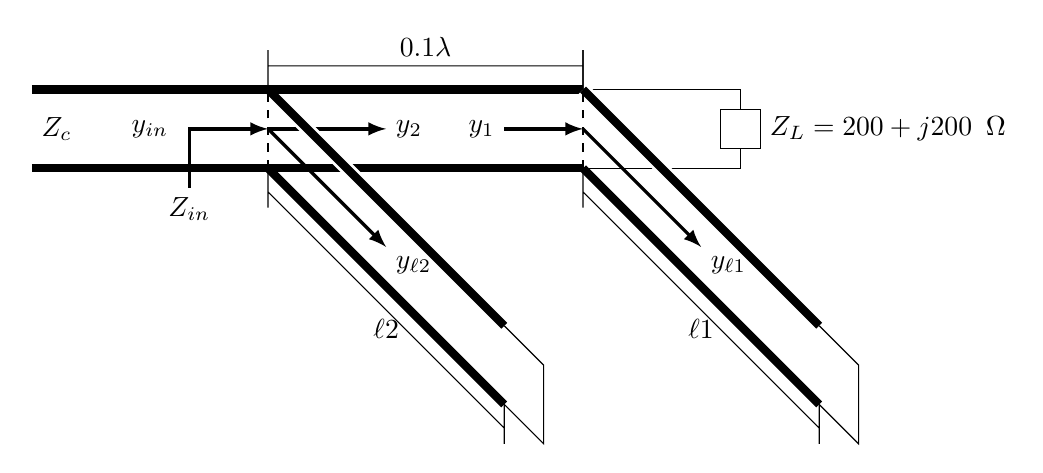
\begin{tikzpicture}[
	scale=1,
	vector/.style={very thick,->, >=latex},
	axis/.style={very thick, ->, >=stealth'}]
		\draw[line width=3pt] (-3,1)--(4,1);
		\draw[line width=3pt] (-3,0)--(4,0);
		\draw[shift={(1.5,0)}] (2,1)--(4.5,1)--(4.5,0)--(2,0);
		\draw[shift={(1.5,0)},fill=white] (4.25,0.75) rectangle (4.75,0.25);
		\draw[shift={(1.5,0)}] (4.75,0.5) node[right]{$Z_L=200+j200\enspace\Omega$};
		\draw (-3,0.5) node[right]{$Z_c$};
		\draw (-1.5,0.5) node{$y_{in}$};
		\draw[vector] (-1,-0.25)|-(0,0.5);
		\draw (-1,-0.25) node[below]{$Z_{in}$};
		\draw [vector] (0,.5)--(1.5,.5);
		\draw[white,line width=5pt] (4,1)--(6,-1);
		\draw[white,line width=5pt] (.4,.6)--(2,-1);
		\draw[line width=3pt] (0,1)--(3,-2);
		\draw[line width=3pt] (0,0)--(3,-3);
		\draw (3,-3)--(3.5,-3.5)--(3.5,-2.5)--(3,-2);
		\draw[shift={(4,0)}] (3,-3)--(3.5,-3.5)--(3.5,-2.5)--(3,-2);
		\draw[shift={(4,0)},line width=3pt] (0,1)--(3,-2);
		\draw[shift={(4,0)},line width=3pt] (0,0)--(3,-3);
		\draw[shift={(4,0)}] (0,0)--(0,-.5) (3,-3)--(3,-3.5) (0,1)--(0,1.5) (0,-0.3)--(3,-3.3);
		\draw[shift={(4,0)}] (1.5,-1.8) node [below] {$\ell1$};
		\draw (0,0)--(0,-.5) (3,-3)--(3,-3.5) (0,1)--(0,1.5) (4,1)--(4,1.5) (4,1.3)--(0,1.3) (0,-0.3)--(3,-3.3);
		\draw (2,1.3) node [above] {$0.1\lambda$} (1.5,-1.8) node [below] {$\ell2$};
		\draw[dashed] (0,0)--(0,1);
		\draw[dashed,shift={(4,0)}](0,0)--(0,1);
		\draw[vector] (0,0.5)--(1.5,-1);
		\draw[shift={(4,0)},vector] (0,0.5)--(1.5,-1);
		\draw (1.5,-1) node [below right] {$y_{\ell2}$};
		\draw [shift={(4,0)}](1.5,-1) node [below right] {$y_{\ell1}$};
		\draw (1.5,0.5) node [right]{$y_2$};
		\draw[vector](3,0.5)--(4,0.5);
		\draw (3,0.5) node [left]{$y_1$};
		

		
\end{tikzpicture}
\caption{Problem 3, parallel double stub tuner, shorts.}
\end{figure}

Normalized load impedance: $z_L=2+j2\Omega$

We want $y_{in} = 1$, so $y_2=1+jB_2$ and $y_{\ell2}=-jB_2$

$y_L=0.250-j0.250$

The two possible $y_1$ admittances are $0.250+j0.575$ and $0.250+j2.15$

By $y_1=y_{\ell1}+y_L$, these two admittances correspond to $y_{\ell1}=j0.825$ and  $y_{\ell1}=j2.40$

$y_{\ell1}=j0.825$ is the closest to the short. This is 0.109+0.250 away from the short.
\[\boxed{\ell_1=0.359\lambda}\]

rotating through, $y_1$ maps onto $y_2$, which the smith chart says $y_2=1+j1.9\Omega$

This means we want $y_{\ell2} = -j1.9$

And we find that 
\[\boxed{\ell_2=0.078\lambda}\]

\begin{figure}[!hbp]
\centering
\begin{tikzpicture}[
	scale=1,
	vector/.style={very thick,->, >=latex},
	axis/.style={very thick, ->, >=stealth'}]
		%	SMITH CHART: 
		%	2.34pt/mm	210pt, outer-mid	201pt, outer-inmid	225pt, outer	192pt, inner	
		%	[thick](90:226pt)--(90:238pt)		
		\node[inner sep=0pt] (russell) at (0,0){\includegraphics[width=1\textwidth]{SMITHCHARTSCAN.jpg}};
		\begin{scope}[shift={(-4.8pt,35.2pt)}]
			\draw[dashed, red, very thick] (30-180:250pt)--(30:250pt) (0,0)--(101:250pt) (0,0)--(-55.5:250pt);
			\draw[dashed, red, very thick, vector](118.25:132pt) arc (118.25:118.25-72:132pt);
			\draw[fill=red] (72:95.5pt) circle(2pt);
			\draw[red] (101:250pt) node[above]{$0.25 + 0.109$};
			\draw[red] (-55.5:250pt) node[below]{$0.328$};
			\draw[dashed, red, very thick] (72:95.5pt) circle (95.5pt);
			\draw[fill=blue] (118.25:132pt) circle (2pt) (118.25:132pt) node [above left]{$\mathbf{y_1}$};
			\draw[fill=blue] (118.25-72:132pt) circle (2pt) (118.25-72:132pt) node [below left]{$\mathbf{y_2}$};
			\draw[fill=blue] (49.75:176pt) circle (2pt)(49.75:176pt) node [right]{$\mathbf{y_1}$};
			\draw[red] (13.25-180:250pt) node [left]{};
			\draw[fill=green] (30:119pt) circle(2pt) (30:119pt) node [below]{$\mathbf{z_L}$};
			\draw[fill=yellow ](30-180:119pt) circle(2pt) (30-180:119pt) node [below]{$\mathbf{y_L}$};
			\draw[fill=yellow ](101:192pt) circle(2pt) (101:192pt)  node [above right]{$\mathbf{y_{\ell1}}$};
			\draw[fill=yellow ](-55.5:192pt) circle(2pt) (-55.5:192pt)  node [below left]{$\mathbf{y_{\ell2}}$};
		\end{scope}
\end{tikzpicture}
\caption{Problem 3, Smith Chart.}
\end{figure}
\subitem{\bf\large (b)}If both stubs are open-circuited, determine stub lengths.
In this case, the same admittance values apply, but this time we rotate the stubs to the left horizontal instead of the right horizontal.

so,

\[\boxed{\ell_1=0.109\lambda \qquad \ell_2=0.328\lambda}\]
%	4
\newpage
\item[{\bf \large 4.}]
(I SWAPPED THE LOAD'S REAL AND IMAGINARY PARTS TO ACHIEVE THE OBJECTIVE OF THIS PROBLEM..)

The parallel double stub tuner will not work to match a $Z_L=25+j12.5\Omega$ load impedance to a $Z_c=100\Omega$ lossless transmission line with stub spacing $d=\lambda/8$, and the first stub connected directly in parallel with the load. It will work however, if we add a little bit of transmission line in between the load and the first stub, call this length $d_L$.
\begin{figure}[!hbp]
\centering
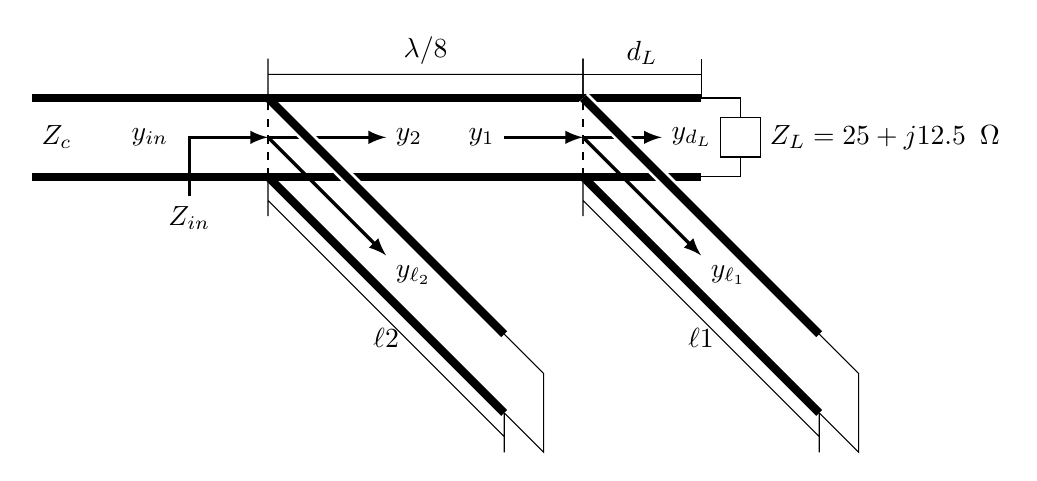
\begin{tikzpicture}[
	scale=1,
	vector/.style={very thick,->, >=latex},
	axis/.style={very thick, ->, >=stealth'}]
		\draw[line width=3pt] (-3,1)--(4,1);
		\draw[line width=3pt] (-3,0)--(4,0);
		\draw[line width=3pt] (4,0)--(5.5,0);
		\draw[line width=3pt] (4,1)--(5.5,1);
		\draw (5.5,1)--(5.5,1.5) (5.5,1.3)--(4,1.3);
		\draw[vector] (4,0.5)--(5,0.5);
		\draw (4.75,1.3) node[above]{$d_L$} (5,0.5) node[right]{$y_{d_L}$};
		\draw[shift={(1.5,0)}] (2,1)--(4.5,1)--(4.5,0)--(2,0);
		\draw[shift={(1.5,0)},fill=white] (4.25,0.75) rectangle (4.75,0.25);
		\draw[shift={(1.5,0)}] (4.75,0.5) node[right]{$Z_L=25+j12.5\enspace\Omega$};
		\draw (-3,0.5) node[right]{$Z_c$};
		\draw (-1.5,0.5) node{$y_{in}$};
		\draw[vector] (-1,-0.25)|-(0,0.5);
		\draw (-1,-0.25) node[below]{$Z_{in}$};
		\draw [vector] (0,.5)--(1.5,.5);
		\draw[white,line width=5pt] (4,1)--(6,-1);
		\draw[white,line width=5pt] (.4,.6)--(2,-1);
		\draw[line width=3pt] (0,1)--(3,-2);
		\draw[line width=3pt] (0,0)--(3,-3);
		\draw (3,-3)--(3.5,-3.5)--(3.5,-2.5)--(3,-2);
		\draw[shift={(4,0)}] (3,-3)--(3.5,-3.5)--(3.5,-2.5)--(3,-2);
		\draw[shift={(4,0)},line width=3pt] (0,1)--(3,-2);
		\draw[shift={(4,0)},line width=3pt] (0,0)--(3,-3);
		\draw[shift={(4,0)}] (0,0)--(0,-.5) (3,-3)--(3,-3.5) (0,1)--(0,1.5) (0,-0.3)--(3,-3.3);
		\draw[shift={(4,0)}] (1.5,-1.8) node [below] {$\ell1$};
		\draw (0,0)--(0,-.5) (3,-3)--(3,-3.5) (0,1)--(0,1.5) (4,1)--(4,1.5) (4,1.3)--(0,1.3) (0,-0.3)--(3,-3.3);
		\draw (2,1.3) node [above] {$\lambda/8$} (1.5,-1.8) node [below] {$\ell2$};
		\draw[dashed] (0,0)--(0,1);
		\draw[dashed,shift={(4,0)}](0,0)--(0,1);
		\draw[vector] (0,0.5)--(1.5,-1);
		\draw[shift={(4,0)},vector] (0,0.5)--(1.5,-1);
		\draw (1.5,-1) node [below right] {$y_{\ell_2}$};
		\draw [shift={(4,0)}](1.5,-1) node [below right] {$y_{\ell_1}$};
		\draw (1.5,0.5) node [right]{$y_2$};
		\draw[vector](3,0.5)--(4,0.5);
		\draw (3,0.5) node [left]{$y_1$};
\end{tikzpicture}
\caption{Problem 4, parallel double stub tuner, shorts.}
\end{figure}
\subitem{\bf\large (a)} What  minimum required additional length $d_L$ do we need to match this load?

The normalized load impedance: $z_L=0.25+j0.125\Omega$ and $y_L=2-j1.9$

From the Smith Chart, the minimum length $d_L$ is
\[\boxed{d_L=0.021\lambda}\]
\\subitem{\bf\large (b)} And the stub lengths will have to be
$y_1=2+j$

$y_{\ell1}=(2+j) - (2-j1.9) = j2.9$ 

After rotating eighth a wavelength, $y_2=1-j$ thus we want the second stub admittance to be $+j$

\[\boxed{\ell_1=0.447\lambda \qquad \ell_2=0.375\lambda}\]
\begin{figure}[!hbp]
\centering
\begin{tikzpicture}[
	scale=1,
	vector/.style={very thick,->, >=latex},
	axis/.style={very thick, ->, >=stealth'}]
		%	SMITH CHART: 
		%	2.34pt/mm	210pt, outer-mid	201pt, outer-inmid	225pt, outer	192pt, inner	
		%	[thick](90:226pt)--(90:238pt)		
		\node[inner sep=0pt] (russell) at (0,0){\includegraphics[width=1\textwidth]{SMITHCHARTSCAN.jpg}};
		\begin{scope}[shift={(-4.8pt,35.2pt)}]
			\draw[dashed, red, very thick] (165.5-180:250pt)--(165.5:116pt) (0,0)--(165.5-195:250pt) (0,0)--(0:250pt) (0,0)--(38.5:250pt) (0,0)--(90:250pt);
			\draw[fill=red] (90:95.5pt) circle(2pt);
			\draw[dashed, red, very thick] (90:95.5pt) circle (95.5pt);
			\draw[red,dashed,vector, very thick,shift={(128pt,0)}] (-110:64pt)arc  (-110:-218:64pt);
			\draw[red,dashed,vector, very thick] (165.5-180:116pt)arc (165.5-180:165.5-195:116pt);
			\draw[red,dashed,vector, very thick]  (26.75:86pt)arc (26.75:26.75-90:86pt);
			\draw[fill=blue] (26.75-90:86pt)circle (2pt)(26.75-90:86pt)node [below left]{$\mathbf{y_2}$};
			\draw[fill=blue] (26.75:86pt) circle (2pt)(26.75:86pt)node [right]{$\mathbf{y_1}$};
			\draw[red] (165.5-180:250pt) node [right]{0.271};
			\draw[red] (165.5-195:250pt) node [right]{0.292};
			\draw[red] (38.5:250pt) node [right]{0.250+0.197=0.447};
			\draw[red] (90:250pt) node [right]{0.250+0.125=0.375};
			\draw[fill=green] (165.5:116pt) circle(2pt) (165.5:116pt) node [below]{$\mathbf{z_L}$};
			\draw[fill=yellow ](165.5-180:116pt) circle(2pt) (165.5-180:116pt) node [above]{$\mathbf{y_L}$};
			\draw[fill=yellow ](165.5-195:116pt) circle(2pt) (165.5-195:116pt) node [below]{$\mathbf{y_{dL}}$};
			\draw[fill=orange](38.5:192pt) circle(2pt) (38.5:192pt) node [below right]{$\mathbf{y_{\ell1}}$};
			\draw[fill=orange](90:192pt) circle(2pt) (90:192pt) node [below right]{$\mathbf{y_{\ell2}}$};
		\end{scope}
\end{tikzpicture}
\caption{Problem 4, Smith Chart.}
\end{figure}
%	5
\newpage
\item[{\bf \large 5.}]
Figure out the ``forbidden zones'' for load impedances with the double stub tuner for the distance $d = \lambda/16$, $\lambda/8$, and $\lambda/4$.
\begin{figure}[!hbp]
\centering
\begin{tikzpicture}[
	scale=1,
	vector/.style={very thick,->, >=latex},
	axis/.style={very thick, ->, >=stealth'}]
		%	SMITH CHART: 
		%	2.34pt/mm	210pt, outer-mid	201pt, outer-inmid	225pt, outer	192pt, inner	
		%	[thick](90:226pt)--(90:238pt)		
		\node[inner sep=0pt] (russell) at (0,0){\includegraphics[width=1\textwidth]{SMITHCHARTSCAN.jpg}};
		\begin{scope}[shift={(-4.8pt,35.2pt)}]
			\filldraw[orange,fill opacity=.3] (0:95.5pt) circle (95.5pt);
			\filldraw[red,fill opacity=.4] (0:128pt) circle (64pt);
			\filldraw[purple,fill opacity=.4] (0:167pt) circle (25pt);
			\draw[dashed, red, very thick] (90:95.5pt) circle (95.5pt);
			\draw[dashed, orange, very thick] (180:95.5pt) circle (95.5pt);
			\draw[dashed, purple, very thick] (45:95.5pt) circle (95.5pt);
			\draw (0:167pt) node {$\mathbf{\lambda/16}$};
			\draw (20:128pt) node {$\mathbf{\lambda/8}$};
			\draw (50:64pt) node {$\mathbf{\lambda/4}$};

		\end{scope}
\end{tikzpicture}
\caption{Problem 5, Smith Chart.}
\end{figure}
\end{enumerate}
\end{spacing}
\end{document}




\begin{IEEEeqnarray*}{lrCl}
\comm{}&
&=&	\\
\comm{}&
&=&	\\
\comm{}&
&=&	\\
\end{IEEEeqnarray*}
	















